\chapter{Materiais e Métodos}



 Devido a área de estudos de ligas de alta entropia ser algo relativamente novo, o número de bases de dados publicamente disponíveis para uso ainda é escasso. Para o atual trabalho foi escolhida uma base de dados disponibilizada em \cite{borg2020expanded} %\cite{qiao2021focused} e \cite{couzinie2018comprehensive}%.
 Essa base representa as características de diferentes ligas de alta entropia, sua composição química, microestrutura, tratamento mecânico, entropia de mistura, raio atômico e outras variáveis que serão descritas a seguir.


\section{Variáveis Utilizadas}\label{sec:MAT_MET_SEC_A}

Na base de dados foram utilizadas as características:


\begin{itemize}
    \item $\Delta S_{mix}$ :  Entropia de mistura
    \item $a_{m}$ :  Constante de rede calculada pela regra das misturas
    \item $ T_{m}$ :  Temperatura de fusão calculada pela regra das misturas
    \item $\chi_{m} $:  Média da eletronegatividades de Pauling
    \item $r_{m} $ :  Raio atômico médio
    \item $\Delta \chi$ :  Média das eletronegatividades de Pauling
    \item $\Delta a$ :  Diferença das das constantes de rede
    \item $\Delta T$ :  Diferença das temperaturas de fusão
    \item $\Delta r$ : Diferença no raio atômico
\end{itemize}

Uma análise exploratória dos dados foi realizada para compreender a estrutura, dispersão, e a correlação entre as variáveis antes que qualquer tipo de tratamento.



\section{Tratamento dos dados}\label{sec:MAT_MET_SEC_B}
\subsection{Tipologia das variáveis}\label{sec:MAT_MET_SEC_B_SUB_A}

Após realizar uma análise exploratória dos dados, verificou-se a presença de variáveis categóricas ou qualitativas nominais, isto é, dados que possuem uma descrição e não um valor numérico contínuo\cite{pinheiro2013probabilidade}. Para tornar esses dados algebricamente manipuláveis, foi realizado um processamento em que as variáveis categóricas são agrupadas, cada grupo recebe um valor numérico, e assim temos as qualitativas nominais como variáveis numéricas discretas\cite{pinheiro2013probabilidade}. 

\subsection{Tratando os dados vazios}\label{sec:MAT_MET_SEC_B_SUB_B}

O conjunto de dados possui valores do tipo ``vazio'' nos atributos de composição química, para um algoritmo de aprendizado de máquina não é possível ajustar uma curva com a presença desse tipo de dado. Neste caso, para tornar esses dados algebricamente manipuláveis, os valores foram substituídos por zero, por exemplo, uma liga de Co1Fe1Ni1 possui apenas informações para os elementos Co, Fe e Ni, sendo assim para essa liga, os outros parâmetros de composição química como por exemplo Al, Cu, Mn recebem o valor zero, ao invés de uma informação vazia. Atribuir por padrão o valor zero nas composições químicas é completamente aceitável, pois é o mesmo que descrever a ausência deste elemento para essa liga.





\subsection{Tratando os dados duplicados}\label{sec:MAT_MET_SEC_B_SUB_C}
Dados faltantes são de certa forma um problema, e também deve-se observar a presença de dados redundantes, isto é, dados duplicados. Quando temos uma quantidade significante de dados repetidos, é possível ocorrer uma análise análise enviesada. A distribuição da microestrutura das ligas apresenta um certo desbalanceamento, mais de 50\% dos dados estão concentrados entre as microestruturas BCC e FCC (figura \ref{fig:distribuicao_microestruturas}), .

\begin{figure}[ht]
    \centering
    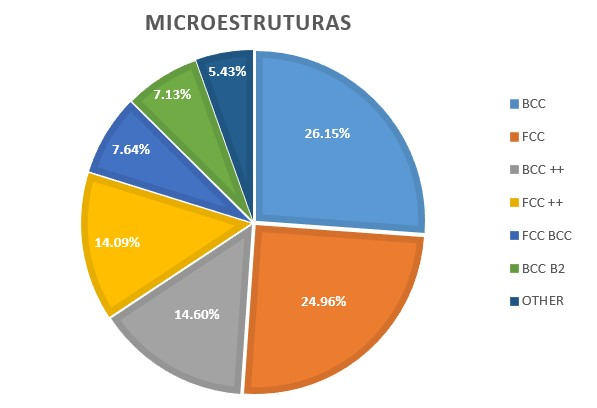
\includegraphics[height=6cm]{distribuicao_microestruturas.jpg} 
    \caption{Distribuição das microestruturas dos dados  }
    \label{fig:distribuicao_microestruturas}
\end{figure}
\FloatBarrier


\begin{figure}[ht]
    \centering
    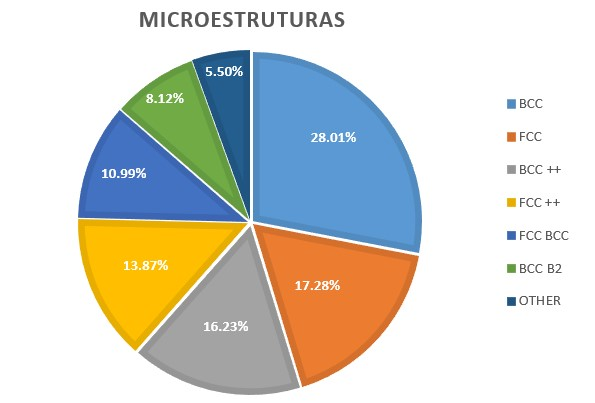
\includegraphics[height=6cm]{distribuicao_microestruturas_sem_duplicados.jpg} 
    \caption{Distribuição das microestruturas dos dados sem duplicados  }
    \label{fig:distribuicao_microestruturas_sem_duplicados}
\end{figure}
\FloatBarrier


Foi feita uma avaliação inicial para verificar a influência da remoção dos dados duplicados na acurácia e no f1-score, os resultados foram gerados utilizando o modelo Random Forest Classifier com as configurações padrão do modelo, também foi realizada a validação cruzada ao treinar o modelo. Após remover informações duplicadas do conjunto de dados a acurácia reduziu aproximadamente 4\%, de forma semelhante, a média do f1-score também reduziu aproximadamente 4\%. Vale ressaltar que a microestrutura FCC apresentou maior impacto na redução do f1-score. Os resultados obtidos estão nas Tabelas \ref{table:relatorio_todos_dados} e \ref{table:relatorio_sem_duplicados}.


\begin{table}[htb]
\centering
\caption{Classificação do conjunto dados completo, n=589 }
\begin{supertabular}{l|c|c|c}
\hline
{ microestruturas } & { precisão } & { recall } & { f1-score } \\\hline
{ CCC } &           {0.7500} &  {0.7402} & {0.7450} \\\hline
{ CCC ++ } &        {0.5070} &  {0.4186} & {0.4585} \\\hline
{ CCC B2 } &        {0.4285} &  {0.5714} & {0.4897} \\\hline
{ CFC } &           {0.7115} &  {0.7551} & {0.7326} \\\hline
{ CFC ++ } &        {0.5967} &  {0.4457} & {0.5103} \\\hline
{ CFC CCC } &       {0.5000} &  {0.6000} & {0.5454} \\\hline
{ OUTROS } &         {0.4736} &  {0.5625} & {0.5142} \\\hline
{ acurácia } &      {0.6230} &  {0.6230} & {0.6230} \\\hline

\end{supertabular}
    \legend{}
    \label{table:relatorio_todos_dados}
\end{table}

\pagebreak



\begin{table}[htb]
\centering
\caption{Classificação após remoção de duplicados, n=382}
\begin{supertabular}{l|c|c|c}
\hline
{ microestruturas } & { precisão } & { recall } & { f1-score } \\\hline
{ CCC } &           {0.7304} &  {0.7850} & {0.7567} \\\hline
{ CCC ++ } &        {0.5416} &  {0.3939} & {0.4561} \\\hline
{ CCC B2 } &        {0.4473} &  {0.5483} & {0.4927} \\\hline
{ CFC } &           {0.5200} &  {0.6290} & {0.5693} \\\hline
{ CFC ++ } &        {0.5813} &  {0.4716} & {0.5208} \\\hline
{ CFC CCC } &       {0.5348} &  {0.5476} & {0.5411} \\\hline
{ OUTROS } &         {0.4500} &  {0.4285} & {0.4390} \\\hline
{ acurácia } &      {0.5837} &  {0.5837} & {0.5837} \\\hline
\end{supertabular}
    \legend{}
    \label{table:relatorio_sem_duplicados}
\end{table}



Após remover os dados duplicados, foi realizada uma análise de correlação Kendalls's (Figura \ref{fig:kendals_correlacao_sem_duplicados}), com finalidade de verificar as variáveis que possuem correlação direta ou inversa. Os elementos Al, Co, Fe, Ni, Si, Cr e Mn possuem uma correlação negativa com os elementos Nb, Mo Ti, Cu V, Zr, Ta, Hf, W.


\begin{figure}[ht]
    \centering
    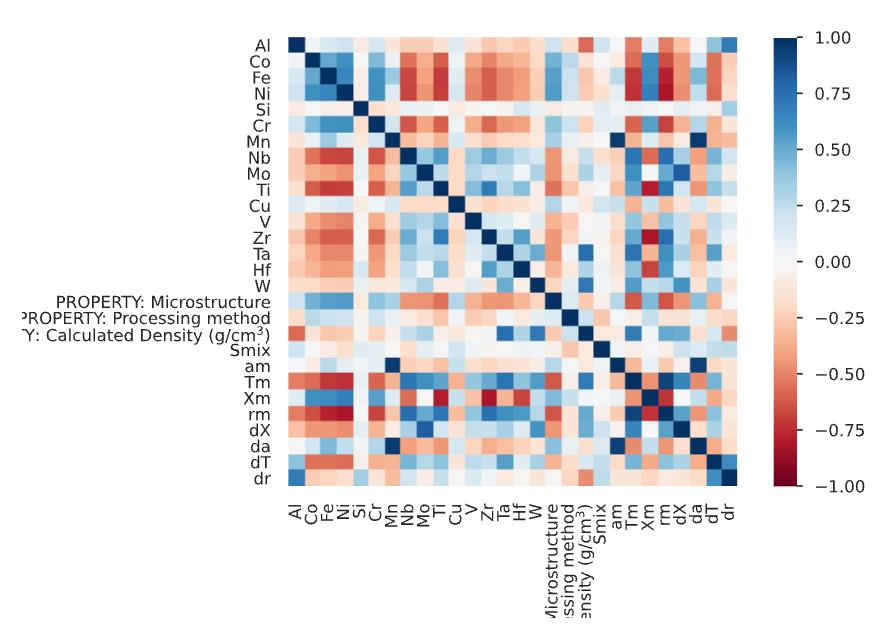
\includegraphics[height=8cm]{estrutura_dos_dados.jpg} 
    \caption{Correlação de Kendall's }
    \label{fig:kendals_correlacao_sem_duplicados}
\end{figure}
\FloatBarrier


\subsection{Normalização dos dados}\label{sec:MAT_MET_SEC_B_SUB_D}

Após remover os itens duplicados do conjunto de dados, foi verificado a redução da acurácia do modelo, que é justificado devido a algum tipo de overfitting do modelo, a ocorrência de dados duplicados são os principais responsáveis por ``viciar'' o modelo a determinado tipo de dado.

A próxima etapa será executada com o conjunto de dados sem os dados duplicados. Primeiramente precisamos subdividir as variáveis em normalizáveis e não normalizáveis. As variáveis normalizáveis são as que possuem alguma possibilidade de conter dados outliers, isto é, dados fora de um intervalo interquartil. Os dados não normalizáveis são os dados de composição química que são percentuais, logo estão dentro do intervalo de 0 a 100\%, e os dados de método de processamento que são categóricos.

Após normalizar os dados, foi feito uma avaliação semelhante ao processo anterior de remoção de dados duplicados, utilizando o modelo RandomForest Classifier com as configurações padrão do modelo e validação cruzada, os resultados encontram se na Tabela \ref{table:relatorio_normalizados}.

\begin{table}[htb]
\centering
\caption{Classificação após normalização de dados}
\begin{supertabular}{l|c|c|c}
\hline
{ microestruturas } & { precisão } & { recall } & { f1-score } \\\hline
{ CCC } &           {0.7217} &  {0.7757} & {0.7477} \\\hline
{ CCC ++ } &        {0.5333} &  {0.3636} & {0.4324} \\\hline
{ CCC B2 } &        {0.4358} &  {0.5483} & {0.4857} \\\hline
{ CFC } &           {0.4864} &  {0.5806} & {0.5294} \\\hline
{ CFC ++ } &        {0.5681} &  {0.4716} & {0.5154} \\\hline
{ CFC CCC } &       {0.5348} &  {0.5476} & {0.5411} \\\hline
{ OUTROS } &         {0.5000} &  {0.5238} & {0.5116} \\\hline
% { acurácia } &      {0.5732} &  {0.5732} & {0.5732} \\\hline
\end{supertabular}
    \legend{acurácia=0.5732, média f1-score=0.5376}
    \label{table:relatorio_normalizados}
\end{table}

\subsection{Comparando diferentes modelos}\label{sec:MAT_MET_SEC_B_SUB_E}

Existem diversos tipos de modelos de algoritmos seja para classificar ou prever algum resultado. No atual trabalho serão avaliados os seguintes modelos: RandomForestClassifier, MLPClassifier, KNeighborsClassifier e SVC. Todos estes modelos foram utilizados com as configurações padrão dos hiper-parâmetros. Para comparar os modelos, foram avaliados os critérios de acurácia e f1-score Figura \ref{fig:comparacao_modelos}.


\begin{figure}[ht]
    \centering
    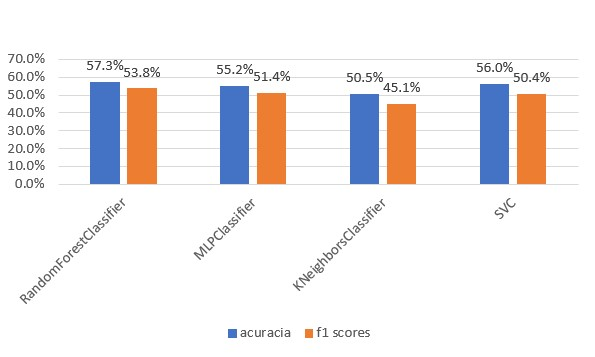
\includegraphics[height=6cm]{comparacao-modelos.jpg} 
    \caption{Acurácia e f1-score de diferentes modelos  }
    \label{fig:comparacao_modelos}
\end{figure}
\FloatBarrier


Foi verificado também a matriz de confusão para cada modelo, com intuito de avaliar a performance da classificação de cada microestrutura.


\begin{figure}[ht]
    \centering
    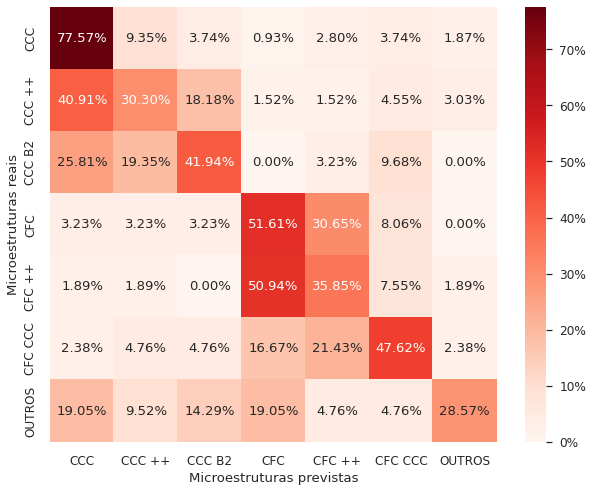
\includegraphics[height=8cm]{KNeighborsClassifier.png} 
    \caption{Matriz de confusão KNN }
    \label{fig:knn_classifier}
\end{figure}
\FloatBarrier

\begin{figure}[ht]
    \centering
    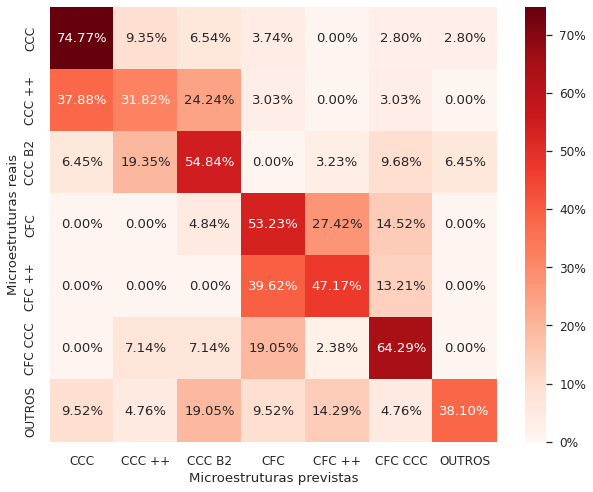
\includegraphics[height=8cm]{MLPClassifier.png} 
    \caption{Matriz de confusão MLP }
    \label{fig:mlp_classifier}
\end{figure}
\FloatBarrier

\begin{figure}[ht]
    \centering
    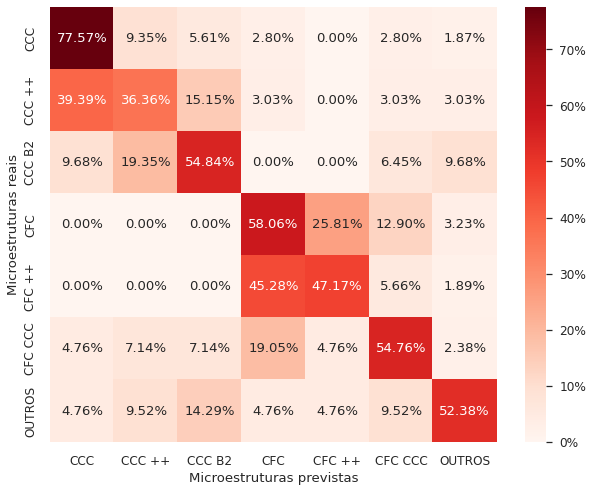
\includegraphics[height=8cm]{RandomForestClassifier.png} 
    \caption{Matriz de confusão Random Forest  }
    \label{fig:random_forest}
\end{figure}
\FloatBarrier

\begin{figure}[ht]
    \centering
    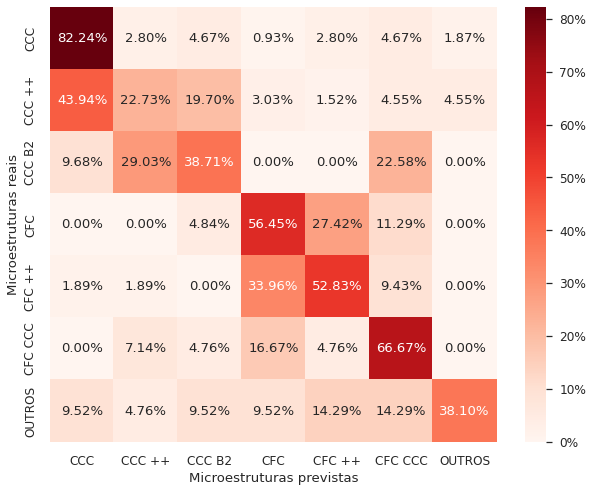
\includegraphics[height=8cm]{SVC.png} 
    \caption{Matriz de confusão SVC  }
    \label{fig:svc_classifier}
\end{figure}
\FloatBarrier





\subsection{Sobreamostragem}\label{sec:MAT_MET_SEC_B_SUB_F}

A linha de pesquisa de ligas de alta entropia ainda é algo recente na comunidade acadêmica, de forma semelhante o utilização dessas informações utilizando ciência de dados e machine learning ainda é algo que está gradativamente se disseminando na comunidade. Por isso a disponibilidade de dados ainda é bastante escassa, para contornar esse desafio, são utilizados modelos que geram novos dados simulados seguindo o mesmo padrão dos dados disponibilizados, fazendo um rebalanceamento dos dados. Foram avaliados diferentes tipos de modelos de sobreamostragem, 

\begin{table}[htb]
\centering
\caption{Resultados de diferentes modelos de sobreamostragem}
\begin{supertabular}{l|c|c}
\hline
{ Modelo de Sobreamostragem }  & { Acurácia } & { média f1-scores } \\\hline
{ SMOTE }                   & {0.8204} & {0.8195} \\\hline
{ ADASYN }                  & {0.7992} & {0.7993} \\\hline
{ BorderlineSMOTE }         & {0.8243} & {0.8240} \\\hline
{ KMeansSMOTE }             & {0.8250} & {0.8254} \\\hline
{ SVMSMOTE }                & {0.8160} & {0.8109} \\\hline

\end{supertabular}
    \legend{}
    \label{table:relatorio_sem_duplicados}
\end{table}
\FloatBarrier

O modelo KMeansSmote apresentou o melhor resultado considerando a sua acuracia e seu f1-score médio, a matriz de confusão conforme a Figura \ref{fig:cm_kmeanssmote}.

\begin{figure}[ht]
    \centering
    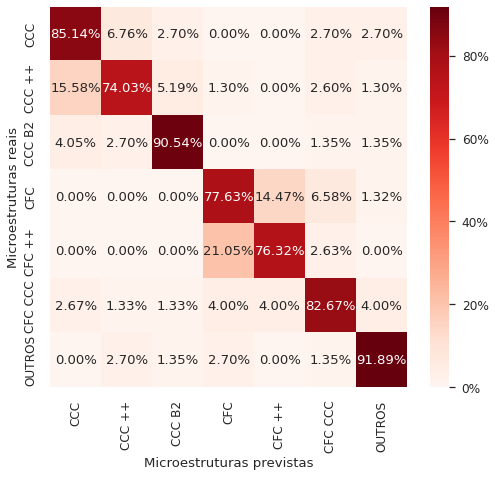
\includegraphics[height=8cm]{KMeansSMOTE.png} 
    \caption{Matriz de confusão de sobreamostragem do modelo KMeansSmote }
    \label{fig:cm_kmeanssmote}
\end{figure}
\FloatBarrier

\subsection{Otimizando hiperparâmetros}\label{sec:MAT_MET_SEC_B_SUB_F}


Após o rebalancear dos dados e decidir o melhor modelo de sobreamostragem, será feita a análise de quais hiperpârametros do modelo Random Forest irá performar melhor para o conjunto de dados. Essa análise é feita a partir de um modelo GridSearchCV \cite{art:grid-search-cv}, que faz uma pesquisa exaustiva sobre valores de parâmetros especificados para um estimador. São passados diferentes parâmetros específicos do modelo que está sendo avaliado, no nosso caso o Random Forest\cite{art:random-forest}, e então o GridSerachCV retorna qual é a melhor combinação de hiperparâmetros informada previamente. Os hiperparâmetros avaliados estão listados abaixo:
\begin{itemize}
\item criterion: entropy, gini;
\item n\_estimators: 50,100,150,200,300,500;
\item max\_depth: 11,12,13,14,15,20,30,40;
\item max\_features: auto, sqrt, log2
\end{itemize}

Das combinações acima, o modelo  GridSearchCV retornou a seguinte combinação de hiperparâmetros:

\begin{itemize}
\item criterion: entropy;
\item n\_estimators: 150;
\item max\_depth: 13;
\item max\_features: auto;
\end{itemize}

O conjunto de dados foi separado numa proporção de 70/30 respectivamente para treino e teste. Sendo assim, após a otimização dos hiperparâmetros, os resultados de classificação estão na Tabela \ref{table:relatorio_otimizados}, estes resultados foram obtidos através de validação cruzada, após sobreamostrar os dados de treino usando o modelo KMeansSmote.


\begin{table}[htb]
\centering
\caption{Classificação após otimizar hiperparâmetros}
\begin{supertabular}{l|c|c|c}
\hline
{ microestruturas } & { precisão } & { recall } & { f1-score } \\\hline
{ CCC } &           {0.7594} &  {0.8108} & {0.7843} \\\hline
{ CCC ++ } &        {0.8309} &  {0.7662} & {0.7972} \\\hline
{ CCC B2 } &        {0.8701} &  {0.9054} & {0.8874} \\\hline
{ CFC } &           {0.7567} &  {0.7368} & {0.7466} \\\hline
{ CFC ++ } &        {0.8133} &  {0.8026} & {0.8079} \\\hline
{ CFC CCC } &       {0.8311} &  {0.8533} & {0.8421} \\\hline
{ OUTROS } &         {0.9041} &  {0.8918} & {0.8979} \\\hline
% { acurácia } &      {0.8231} &  {0.8231} & {0.8231} \\\hline
\end{supertabular}
    \legend{acurácia=0.8231, média f1-score=0.8233}
    \label{table:relatorio_otimizados}
\end{table}


Com o modelo treinado através dos dados sobreamostrados, resta validar se o modelo apresenta uma acurácia satisfatória a partir de um conjunto de dados ainda não visto. Para isso, após treinar o algoritmo com os dados sobreamostrados, será verificado se a classificação dos dados de teste apresenta uma acurácia satisfatória.
\pagebreak
\begin{table}[htb]
\centering
\caption{Classificação após otimizar hiperparâmetros utilizando dados de teste}
\begin{supertabular}{l|c|c|c}
\hline
{ microestruturas } & { precisão } & { recall } & { f1-score } \\\hline
{ CCC } &           {0.7948} &  {0.9393} & {0.8611} \\\hline
{ CCC ++ } &        {0.8000} &  {0.5000} & {0.6153} \\\hline
{ CCC B2 } &        {0.6666} &  {0.6666} & {0.6666} \\\hline
{ CFC } &           {0.5263} &  {0.5555} & {0.5405} \\\hline
{ CFC ++ } &        {0.8181} &  {0.5000} & {0.6206} \\\hline
{ CFC CCC } &       {0.5000} &  {0.8461} & {0.6285} \\\hline
{ OUTROS } &         {0.6000} &  {0.3750} & {0.4615} \\\hline
\end{supertabular}
    \legend{acurácia=0.6782, média f1-score=0.6278}
    \label{table:relatorio_otimizados_validacao}
\end{table}

\pagebreak

